%%%%%%%%%%%%%%%%%%%%%%%%%%%%%%%%%%%%%%%%%%%%%%%%%%%%%%%%%%%%%%%%%%%%%%%%%%%
\section{\label{sec:QualitativeDiscussion}The basic idea: Qualitative discussion}
%%%%%%%%%%%%%%%%%%%%%%%%%%%%%%%%%%%%%%%%%%%%%%%%%%%%%%%%%%%%%%%%%%%%%%%%%%%

This section is intended to introduce the particle physics model used in our analysis and to give a qualitative understanding of its different regimes. Furthermore, we will justify the assumptions that go into the numerical computations.

Our setting introduces one real scalar singlet $S$ (with mass $m_S$) and one right-handed neutrino $N$ (with mass $m_N$) beyond the particle content of the SM.\footnote{In general, any number of right-handed neutrinos can be assumed in this model. In the case of more than one generation, the scalar will then decay into all kinematically accessible right-handed states $N_i$ with branching fractions given by $y_i^2/\sum_k y_k^2$. If the mixing between the different right-handed states is large enough, all right-handed neutrinos will decay into the lightest state ($N_1$ by convention) quickly and the results of this paper stay unaltered under the substitution $y^2 \rightarrow \sum_k y_k^2$. If, however, the mixing inside the sterile sector is small, there might be additional complications due to late injection of highly energetic DM particles by the decay of the heavier states into the lighter ones.} The right-handed neutrino is coupled to the singlet scalar via a Yukawa-type interaction with coupling $y$,
\begin{align}
 \Lag \supset - \frac{y}{2} S \overline{N^c}N + \hc \,,
 \label{eq:YukawaCouplingLagrangia}
\end{align}
while the new scalar singlet is coupled to the Higgs doublet $\Phi$ via the most generic potential symmetric under a global $\mathbb{Z}_4$-symmetry:\footnote{Suitable charge assignments are given by $S \to -S$ and $N\to \pm i N$. For further comments on this assumption, see~\cite{Merle:2013wta,Merle:2015oja} and references therein. The (rather mild) consequences of giving up this simplification are discussed in~\cite{Petraki:2007gq}.}
\begin{align}
  \sub{V}{scalar} =   \frac{1}{2} m_S^2 S^2 + \frac{\lambda_S}{4} S^4 +2\lambda \left(\Phi^\dagger \Phi\right)S^2 \,.
 \label{eq:ScalarPotentialLagrangian}
\end{align}
Accordingly, the complete Lagrangian of the model reads
\begin{align}
  \Lag = \LagArg{SM} + \left[\frac{i}{2}\overline{N} \delslashed N + \frac{1}{2}\left(\partial_\mu S\right)\left(\partial^\mu S\right) - \frac{y}{2}S\overline{N^c}N +\hc \right] - \sub{V}{scalar} + \Lag_\nu \,,
 \label{eq:ModelLagrangian}
\end{align}
where $\Lag_\nu$ is the part of the Lagrangian that can give mass to the active neutrinos. We do \emph{not} assume any vacuum expectation value (VEV) for $S$ in our analysis, however, we will include the constraints which would arise of the VEV of $S$ gave the sterile neutrinos their mass, so that the case of $\langle S \rangle \neq 0$ can be qualitatively recovered from our analysis.

Note that we assume active-sterile mixing to be so small that the contribution from the DW mechanism to the production of sterile neutrinos is negligible compared to the part produced by scalar decay, based on taking into account X-ray limits on the decay of sterile neutrino DM. In Ref.~\cite{Merle:2015vzu} it has been shown that the DW modification to any previously produced population of sterile neutrinos (from whichever main production mechanism) is of a few percent at most, and completely negligible for masses $m_N$ larger than about $\unit{4}{keV}$.

Our setup mainly allows us to produce scalars from their coupling to the SM with interactions of the type $\sub{\overline{X}}{SM}\sub{X}{SM} \leftrightarrow SS$. Subsequently, the scalars decay into sterile neutrinos via $S \rightarrow N N$. We have to distinguish three different regimes:
\begin{enumerate}
 \item[I] Production before the electroweak phase transition (EWPT): all four degrees of freedom of the $SU(2)_L$-doublet Higgs $\Phi$ contribute equally to the production/depletion of scalars from/into the thermal bath.
 \item[II] Production after EWPT with $m_S > m_h/2$, where $m_h$ is the mass of the Higgs after electroweak symmetry breaking. Now the Higgs and the massive gauge bosons interact with the scalar different ways.
 \item[III] Production after EWPT with $m_S < m_h/2$. This is similar to case~II, the difference being that the Higgses present in the thermal plasma are now kinematically allowed to decay into pairs of scalars.
\end{enumerate}

\begin{table}[t!]
 \centering
 \begin{tabular}{|c|cccccc|}
  \hline
  \rotatebox{90}{regime~} & \multicolumn{6}{|c|}{production channels} \\ 
  \hline 
  I & 
  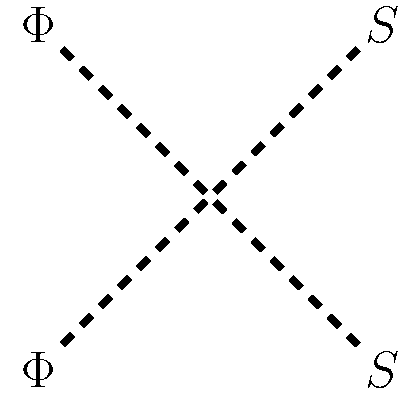
\includegraphics[scale=0.32]{figures/feynman_diagrams/phiphissfeynman.pdf} & & & & &\\
  \hline
  II &
  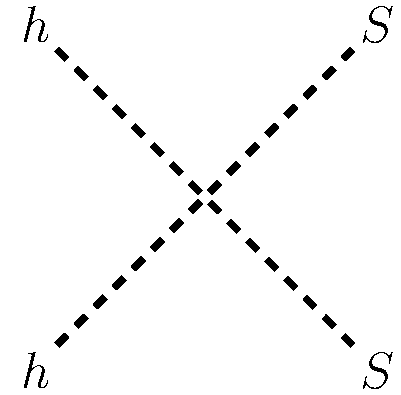
\includegraphics[scale=0.32]{figures/feynman_diagrams/hhssfeynman.pdf} &
  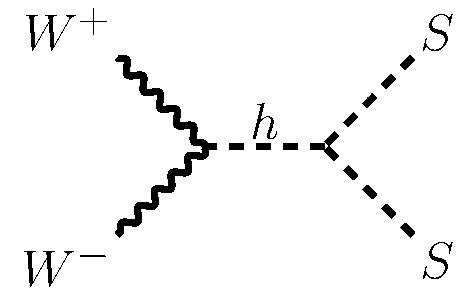
\includegraphics[scale=0.32]{figures/feynman_diagrams/wwssfeynman.pdf} &
  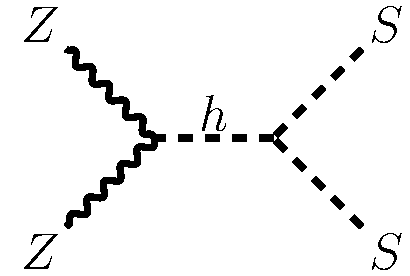
\includegraphics[scale=0.32]{figures/feynman_diagrams/zzssfeynman.pdf} &
  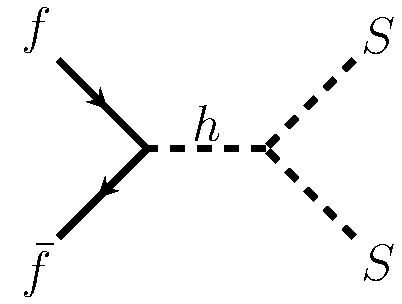
\includegraphics[scale=0.32]{figures/feynman_diagrams/ffssfeynman.pdf} &
  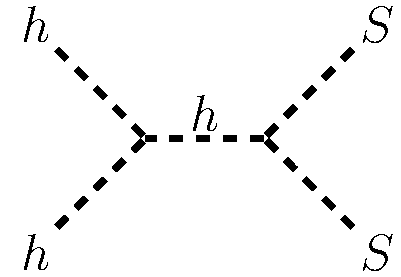
\includegraphics[scale=0.32]{figures/feynman_diagrams/hhssfeynman_s-channel.pdf} & \\
  \hline
  III & 
  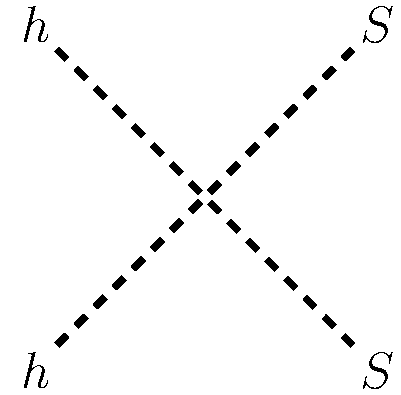
\includegraphics[scale=0.32]{figures/feynman_diagrams/hhssfeynman.pdf} &
  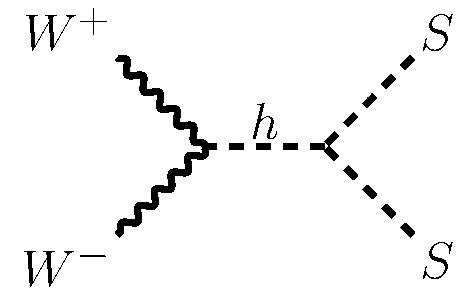
\includegraphics[scale=0.32]{figures/feynman_diagrams/wwssfeynman.pdf} &
  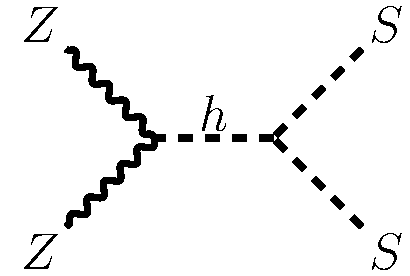
\includegraphics[scale=0.32]{figures/feynman_diagrams/zzssfeynman.pdf} &
  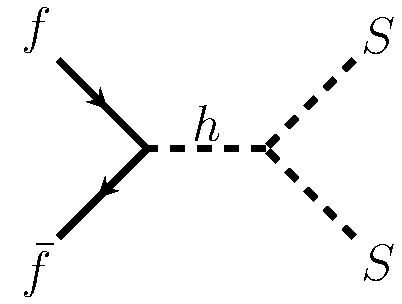
\includegraphics[scale=0.32]{figures/feynman_diagrams/ffssfeynman.pdf} &
  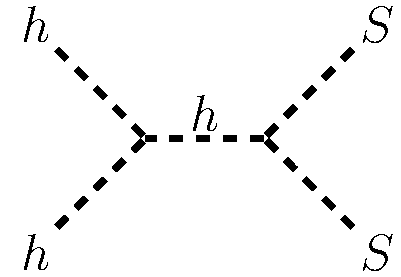
\includegraphics[scale=0.32]{figures/feynman_diagrams/hhssfeynman_s-channel.pdf} & 
  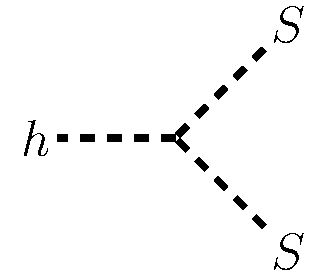
\includegraphics[scale=0.32]{figures/feynman_diagrams/hssfeynman.pdf} \\
  \hline
 \end{tabular}
  \caption{\label{tab:RegimesFeynman}Relevant production channels in regimes~I--III.}
\end{table}

The channels corresponding to regimes I--III are listed in \tabref{tab:RegimesFeynman}. Note that we have omitted the diagrams with a scalar $S$ in the $t$- or the $u$-channels, since they will contribute to the production only at order $\orderof{\lambda^3}$, i.e., suppressed by another small factor of $\lambda$ compared to the leading order. In regimes~II and~III, the fermionic initial state $f$ only receives a contribution from the top quark in practice, since all other channels are suppressed by their small Yukawa couplings. Couplings to lighter fermions may appear relevant at first sight, since in that case the Higgs could potentially be on-shell, which may enhance the cross section by orders of magnitude. However, this case of an on-shell Higgs needs to be subtracted adequately to avoid double-counting of decay events of thermal Higgses~\cite{Frigerio:2011in}, and they ultimately do not contribute much. Note that, at precision level, even thermal corrections to the parameters can play a role~\cite{Drewes:2015eoa}.

In general, production will always start in regime~I and then, unless finished in that regime, proceed either in regime~II or in regime~III after EWPT, depending on the value of $m_S$. In the case of small Higgs portal couplings $\lambda$, the scalar will freeze in. This production mechanism is most efficient when $T \sim m_S$. In the case of larger $\lambda$, the scalar first equilibrates and then freezes out. In this scenario, the freeze-out time will also be linked to $m_S$. Accordingly, there is a finite span in cosmic time (or in the temperature $T$, equivalently) in which the production is effectively taking place. 

This time span is illustrated in \Figref{fig:RegimeExampleCases} for four different masses $m_S$. Red arrows correspond to small Higgs portal couplings $\lambda$, implying that the scalar never equilibrates, but freezes in instead. In this case, we have defined the time span of production starting when 10\% of the final yield $Y$ of a would-be stable scalar is produced and ending when 90\% are produced. Blue arrows indicate the time spans for scalars freezing out before decaying into sterile neutrinos. In this case, there is no physically preferred initial time. Note that, even when assuming a vanishing initial abundance, thermalisation is fast compared to the time scale of the decay. The late-end boundary (i.e., at low temperatures) of the time span is, however, defined by $Y/\sub{Y}{eq}=10$, where $\sub{Y}{eq}$ denotes the equilibrium yield.

One can clearly see that, in cases where $m_S<m_h/2$, the freeze-in of scalars occurs only after EWPT. This can be explained by the fact that the decay of thermal Higgses after EWPT completely dominates the production as soon as this channel is kinematically accessible~\cite{Adulpravitchai:2014xna}. For $m_S=\unit{65}{GeV}$, production sets in before EWPT and stops at temperatures of some tens of $\unitonly{GeV}$. In the case of a much heavier scalar (say, $m_S=\unit{500}{GeV}$), production even ends before EWPT, since the kinetic energies of the Higgses after EWPT are insufficient to produce the heavy scalar. 

Note that we need the particle distribution function of all sourcing species in the plasma, like gauge bosons or Higgses, to account for the production of scalars induced by the channels shown in \tabref{tab:RegimesFeynman}. In general, the dynamics of each of these species is determined by their own Boltzmann equation. Fortunately, it is not necessary to incorporate more than two equations into the system, since we can safely assume these particles to be in thermal equilibrium, an assumption that has been readily made in~\cite{Adulpravitchai:2014xna} even for small $T$, but not proven to work. We have explicitly checked that the Higgs indeed stays in equilibrium at least until $T \approx \unit{1}{GeV}$. Note that the usual estimate for WIMP-like particles of mass $m$ is that freeze-out occurs at $T_\text{freeze-out}\sim m/20$. The reason that the Higgs stays in equilibrium longer are inverse decay processes, and similar arguments apply to the gauge bosons and to the top-quark, cf.\ App.~\ref{app:B:Higgs-FO}. Still, the number densities of all SM particles become strongly Boltzmann-suppressed for temperatures of, say, $10$--$\unit{20}{GeV}$. Hence, production \emph{always} ceases at these temperatures, simply because there are hardly any particle left in the bath, even if they are still in equilibrium.

\begin{figure}
 \centering
 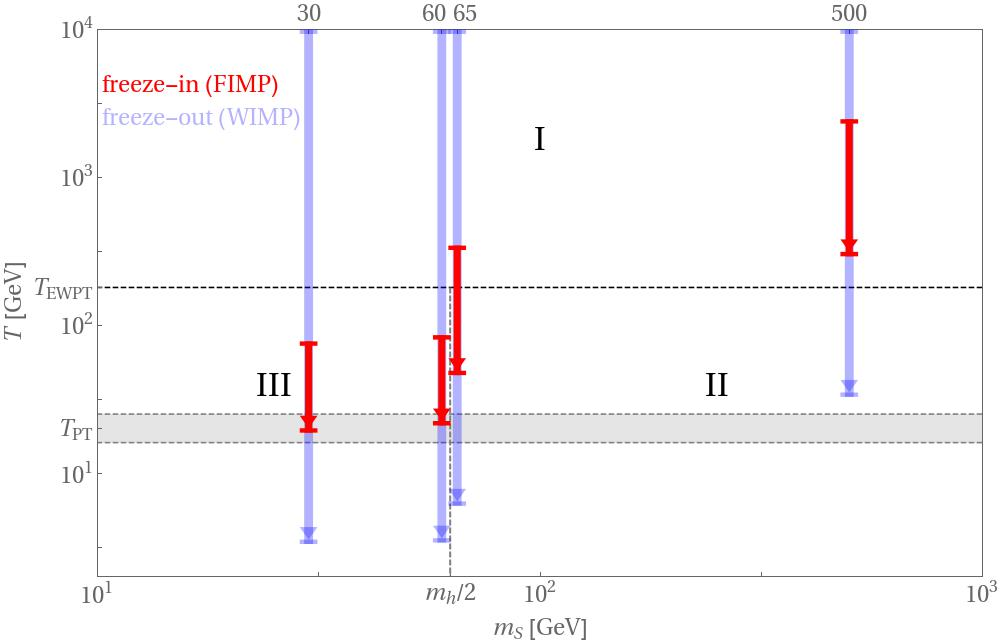
\includegraphics[width=0.8 \textwidth]{figures/mass_regimes_w_WIMP.jpg}
 \caption{\label{fig:RegimeExampleCases}Temperature ranges of the plasma temperature $T \equiv T_\gamma$ at which the scalar singlet $S$ is efficiently produced in the freeze-in scenario (red) and in the freeze-out scenario (light blue). We present four different scalar masses (30, 60, 65, and 500~GeV) that span the variety of possible production times. $\sub{T}{EWPT}$ indicates the temperature when electroweak phase transition happens, while $\sub{T}{PT}$ is supposed to give a rough idea of the temperature when the Higgs and gauge bosons become strongly Boltzmann-suppressed, even if still equilibrated with the remaining SM degrees of freedom.}
\end{figure}



